\newpage
% !TEX TS-program = pdflatex
% !TEX encoding = UTF-8 Unicode

% This is a simple template for a LaTeX document using the "article" class.
% See "book", "report", "letter" for other types of document.

\documentclass[12pt]{article} % use larger type; default would be 10pt

\usepackage[utf8]{inputenc} % set input encoding (not needed with XeLaTeX)

\usepackage[toc,page]{appendix}
\usepackage{amsmath}
\usepackage{amssymb}
\usepackage{inputenc}
%%% Examples of Article customizations
% These packages are optional, depending whether you want the features they provide.
% See the LaTeX Companion or other references for full information.

%%% PAGE DIMENSIONS
\usepackage{geometry} % to change the page dimensions
\geometry{a4paper} % or letterpaper (US) or a5paper or....
% \geometry{margin=2in} % for example, change the margins to 2 inches all round
% \geometry{landscape} % set up the page for landscape
%   read geometry.pdf for detailed page layout information

\usepackage{graphicx} % support the \includegraphics command and options
\usepackage{epstopdf}
\usepackage{import}
\usepackage{float}
\graphicspath{{Graphics/}}
% \usepackage[parfill]{parskip} % Activate to begin paragraphs with an empty line rather than an indent

%%% PACKAGES
\usepackage{booktabs} % for much better looking tables
\usepackage{array} % for better arrays (eg matrices) in maths
\usepackage{paralist} % very flexible & customisable lists (eg. enumerate/itemize, etc.)
\usepackage{verbatim} % adds environment for commenting out blocks of text & for better verbatim
\usepackage{subfig} % make it possible to include more than one captioned figure/table in a single float
\usepackage{hyperref}
\usepackage{datetime}
\usepackage{braket}
% These packages are all incorporated in the memoir class to one degree or another...

%%% HEADERS & FOOTERS
\usepackage{fancyhdr} % This should be set AFTER setting up the page geometry
\pagestyle{fancy} % options: empty , plain , fancy
\renewcommand{\headrulewidth}{0pt} % customise the layout...
\lhead{}\chead{}\rhead{}
\lfoot{}\cfoot{\thepage}\rfoot{}

%%% SECTION TITLE APPEARANCE
\usepackage{sectsty}
\allsectionsfont{\sffamily\mdseries\upshape} % (See the fntguide.pdf for font help)
% (This matches ConTeXt defaults)

%%% ToC (table of contents) APPEARANCE
\usepackage[nottoc,notlof,notlot]{tocbibind} % Put the bibliography in the ToC
\usepackage[titles,subfigure]{tocloft} % Alter the style of the Table of Contents
\renewcommand{\cftsecfont}{\rmfamily\mdseries\upshape}
\renewcommand{\cftsecpagefont}{\rmfamily\mdseries\upshape} % No bold!
\usepackage{color}
%%% END Article customizations

\usepackage{datatool}% http://ctan.org/pkg/datatool
\newcommand{\sortitem}[2][\relax]{%
  \DTLnewrow{list}% Create a new entry
  \ifx#1\relax
    \DTLnewdbentry{list}{sortlabel}{#2}% Add entry sortlabel (no optional argument)
  \else
    \DTLnewdbentry{list}{sortlabel}{#1}% Add entry sortlabel (optional argument)
  \fi%
  \DTLnewdbentry{list}{description}{#2}% Add entry description
}
\newenvironment{sortedlist}{%
  \DTLifdbexists{list}{\DTLcleardb{list}}{\DTLnewdb{list}}% Create new/discard old list
}{%
  \DTLsort{sortlabel}{list}% Sort list
  \begin{itemize}%
    \DTLforeach*{list}{\theDesc=description}{%
      \item \theDesc}% Print each item
  \end{itemize}%
}
\newcommand*{\rom}[1]{\expandafter\@slowromancap\romannumeral #1@}

\usepackage{listings}
\usepackage{color}

\definecolor{dkgreen}{rgb}{0,0.6,0}
\definecolor{gray}{rgb}{0.5,0.5,0.5}
\definecolor{mauve}{rgb}{0.58,0,0.82}

\lstset{frame=tb,
  language=Matlab,
  aboveskip=3mm,
  belowskip=3mm,
  showstringspaces=false,
  columns=flexible,
  basicstyle={\small\ttfamily},
  numbers=none,
  numberstyle=\tiny\color{gray},
  keywordstyle=\color{blue},
  commentstyle=\color{dkgreen},
  stringstyle=\color{mauve},
  breaklines=true,
  breakatwhitespace=true,
  tabsize=3
}


\newcommand{\executeiffilenewer}[3]{%
\ifnum\pdfstrcmp{\pdffilemoddate{#1}}%
{\pdffilemoddate{#2}}>0%
{\immediate\write18{#3}}\fi%
}



\title{User manual of the Coincidence data analysis software (ANACONDA 2)}
%author{}
\date{\today} % Activate to display a given date or no date (if empty),
         % otherwise the current date is printed 

\begin{document}
\maketitle
\tableofcontents
\newpage

This document shows how the data analysis package `ANACONDA 2', or `ANACONDA' can be used. ANACONDA allows the analysis of data recorded in experiments that use single-particle detectors (e.g. ions, electrons, photons ...), for example to study the correlation between these particles. These are often called `\href{https://www.sciencedirect.com/science/article/pii/S0368204815001310}{coincidence}' spectrocopic treatment methods.

%\input{Getting started}
%\section{Metadata}
The metadata contains all the information \emph{about} the data, such as conversion parameters, but also filter and plot parameters. The package comes shipped with `default' parameters, which can be used when the data is first imported by the user. It is recommended to copy the default parameters close to the local files, such that they are not changed, for instance when the package is upgraded.
The default metadata in the package is defined for each spectrometer, since each spectrometer has different numbers of detectors, with different measurement signals (position, time, etc \dots). 

\begin{figure}[H]
   \centering
    \centerline{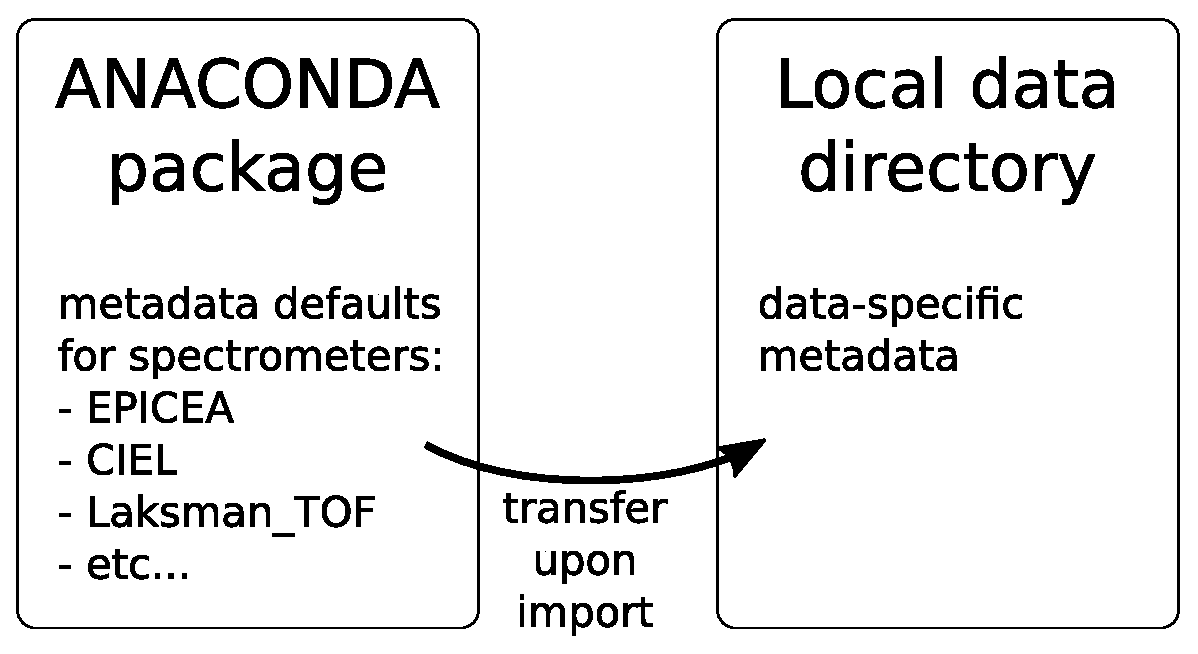
\includegraphics[width=0.7\textwidth]{Graphics/metadata_defaults.eps}}
\caption{Default metadata (or configuration data) are defined in the package, to be copied upon first import of a new data file.}
\label{metadata_defaults}
\end{figure}

\subsection{Metadata structure}
The metadata contains all information needed to correct, convert, fit and visualize the data.
\\
The metadata structure is divided into different categories:
\begin{itemize}
\item[\emph{sample}], e.g. atomic mass, expected fragment masses, constituent masses.
\item[\emph{photon beam}], e.g. the photon energy, intensity, duration, etc
\item[\emph{spectrometer}],  e.g. the name, voltages and relevant dimensions of the used spectrometer are listed here.
\item[\emph{detectors}], e.g. the names and properties of the detectors are stored in here.
\item[\emph{correct}] The parameters needed to execute corrections onto the raw data, before conversion. For example, translation in X and Y to move the centre of detection into the origin of the coordinate system.
\item[\emph{calibrate}] The information needed to perform the calibrations. Note that these are not the actual calibration factors, they are stored in the 'convert' field.
\item[\emph{fit}] The fitting parameters.
\item[\emph{convert}] The conversion factors (sorted in terms of detectors), such as mass to charge conversion.
\item[\emph{plot}] The user-preferred plotstyle.
\end{itemize}

Most fields in the metadata are obvious to understand. We elaborate on a few that might be cause of confusion.

\paragraph{sample}
 We elaborate on the definition difference between 'constituents' and 'fragments' here:
\begin{itemize}
\item Constituents: The building block of which the sample consists. Example: a water-ammonia mixed cluster has consituents water and ammonia
\item Fragments: The expected fragments from the sample. Example: a water-ammonia mixed cluster has the expected fragments of hydrogenated water-ammonia mixed clusters.
\end{itemize}


\subsection {storage}
The metadata is stored as a struct, with the above categories as their fieldnames. 

The metadata, or data settings, belong to a separate datafile. They are stored in a separate file with the same base name as the main datafile (\emph{'filename.mat'}), but with the addition \emph{'md\_.m'} before the filename, so \emph{'md\_filename.m'}. This is done to make it easy to manually copy metadata files to different datafiles. For example: reading the datafile \emph{H2O\_003.mat} will read its metadata from the file \emph{md\_H2O003.m}. The metadata is stored in a plain-text m-file, which makes it possible to read and change parameters from outside MATLAB.

\lstset{language=MATLAB}
\begin{lstlisting}
exp1_md.sample
exp1_md.photon
exp1_md.spec
exp1_md.corr
exp1_md.calib
exp1_md.fit
exp1_md.conv
exp1_md.plot
\end{lstlisting}

%\section{Data flow}
In this section, the transition from raw hits to a calibrated and physically interpretable signal is described. 

\begin{figure}[h]
   \centering
    \centerline{\includegraphics[width=1\textwidth]{Graphics/data_flow.pdf}}
\caption{Example of data flow}
\label{Data_flow}
\end{figure}

%\newpage
\section{The package}
The package is defined as the collection of functions (or `methods') that are part of this software. The methods are divided up in several categories:
\begin{itemize}
\item[\emph{import/output (IO)}]: Data Input/Output functions
\item[\emph{correct}]: Correction of the data, for example abberrations.
\item[\emph{convert}]: Conversion of the corrected data to other variables (signals)
\item[\emph{filter}]: The formation of filters that view only parts of the data
\item[\emph{plot}]: Show histograms of many kinds, and other graphics tools
\item[\emph{calibrate}]: Methods to verify the conversion
\item[\emph{macros}]: Meta-functions that automize the treatment and analysis of (multiple) experiments.
\item[\emph{fit}]: Methods to characterize histograms from models.
\item[\emph{theory}]: Methods to visualize or use (statistical) models.
\item[\emph{general}]: General MATLAB functions used in different places in the package.
\end{itemize}



\newpage
\subsection{Input Output (IO)}
\paragraph{Importing DLT files} The importing of data from DLT files is done with software written by Erik Mansson. 

\paragraph{Importing KoboldPC (LMF) files} Not yet implemented.

\paragraph{handling of multiple files} Not yet implemented.

\subparagraph{Combining two files} Not yet implemented.

\subparagraph{Comparing two files} Not yet implemented.


\newpage
\subsection{correct}
This section lists all the corrections that can be performed. It is logged in the datafile whether a certain correction has already been performed, in the \emph{exp\_name.h.det\_name.corr\_log} field.
First of all, the coordanite system used in this software is defined in Figure \ref{coor_sys}.

\begin{figure}
  \centering
  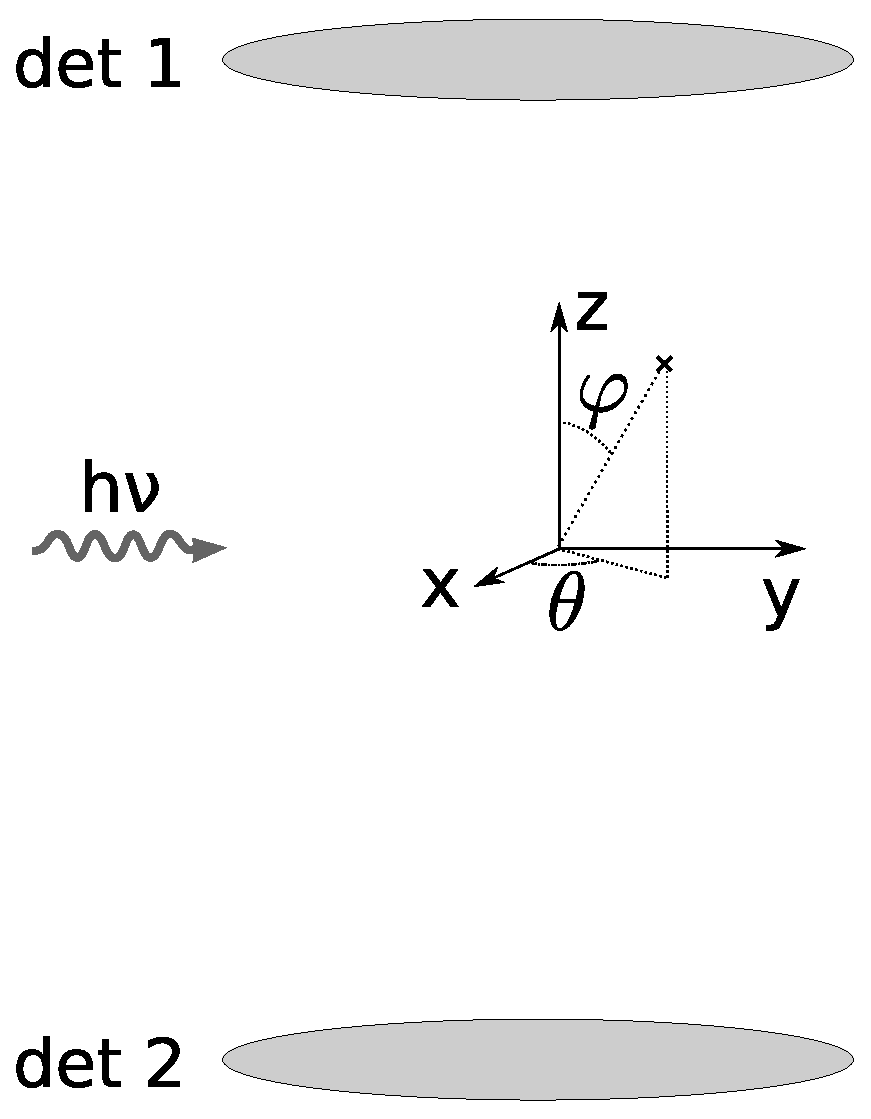
\includegraphics[width=0.5\textwidth]{Graphics/coordinate_system.eps}
  \captionof{figure}{Definition of coordinate system used in this Software. The x-axis aligns with the polarization and the molecular beam, the Y-direction aligns with the photon beam, and Z aligns with the detector axis.}
\label{coor_sys}
\end{figure}

\subsubsection{detection image translation}

\begin{figure}
\centering
\begin{minipage}{.5\textwidth}
  \centering
  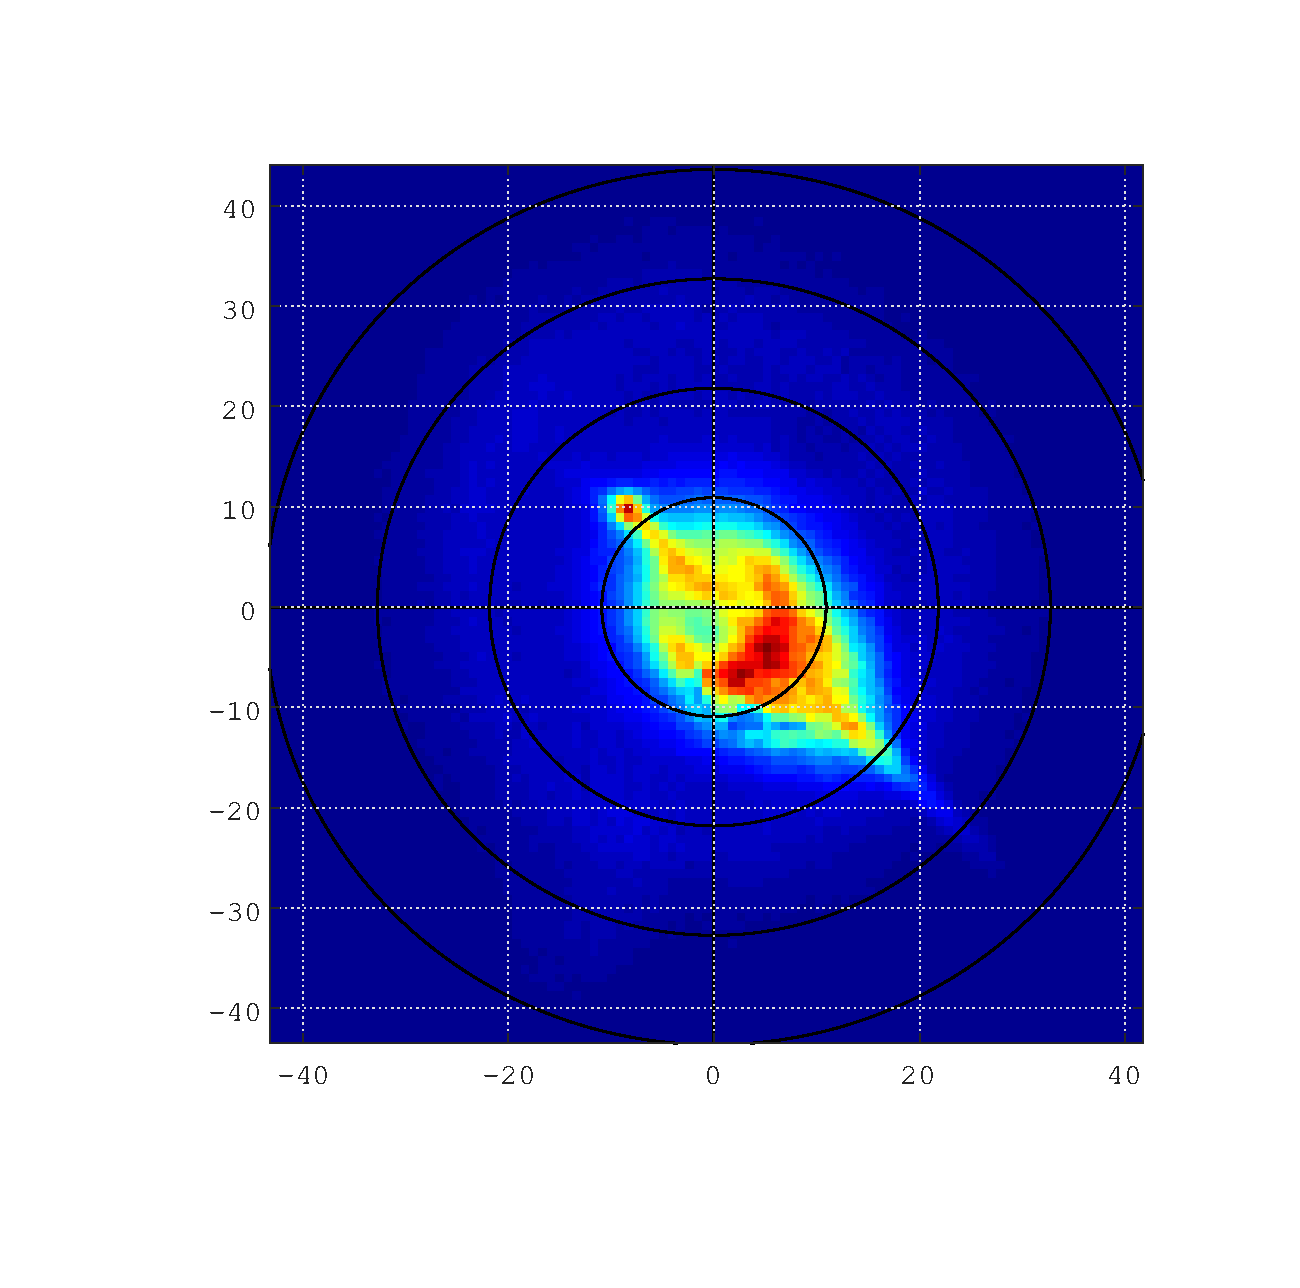
\includegraphics[width=1\textwidth]{Graphics/centre_calibration_before.eps}
  \captionof{figure}{Detector image of all hits before centring}
\label{centre_calibration_before}
\end{minipage}%
\begin{minipage}{.5\textwidth}
  \centering
  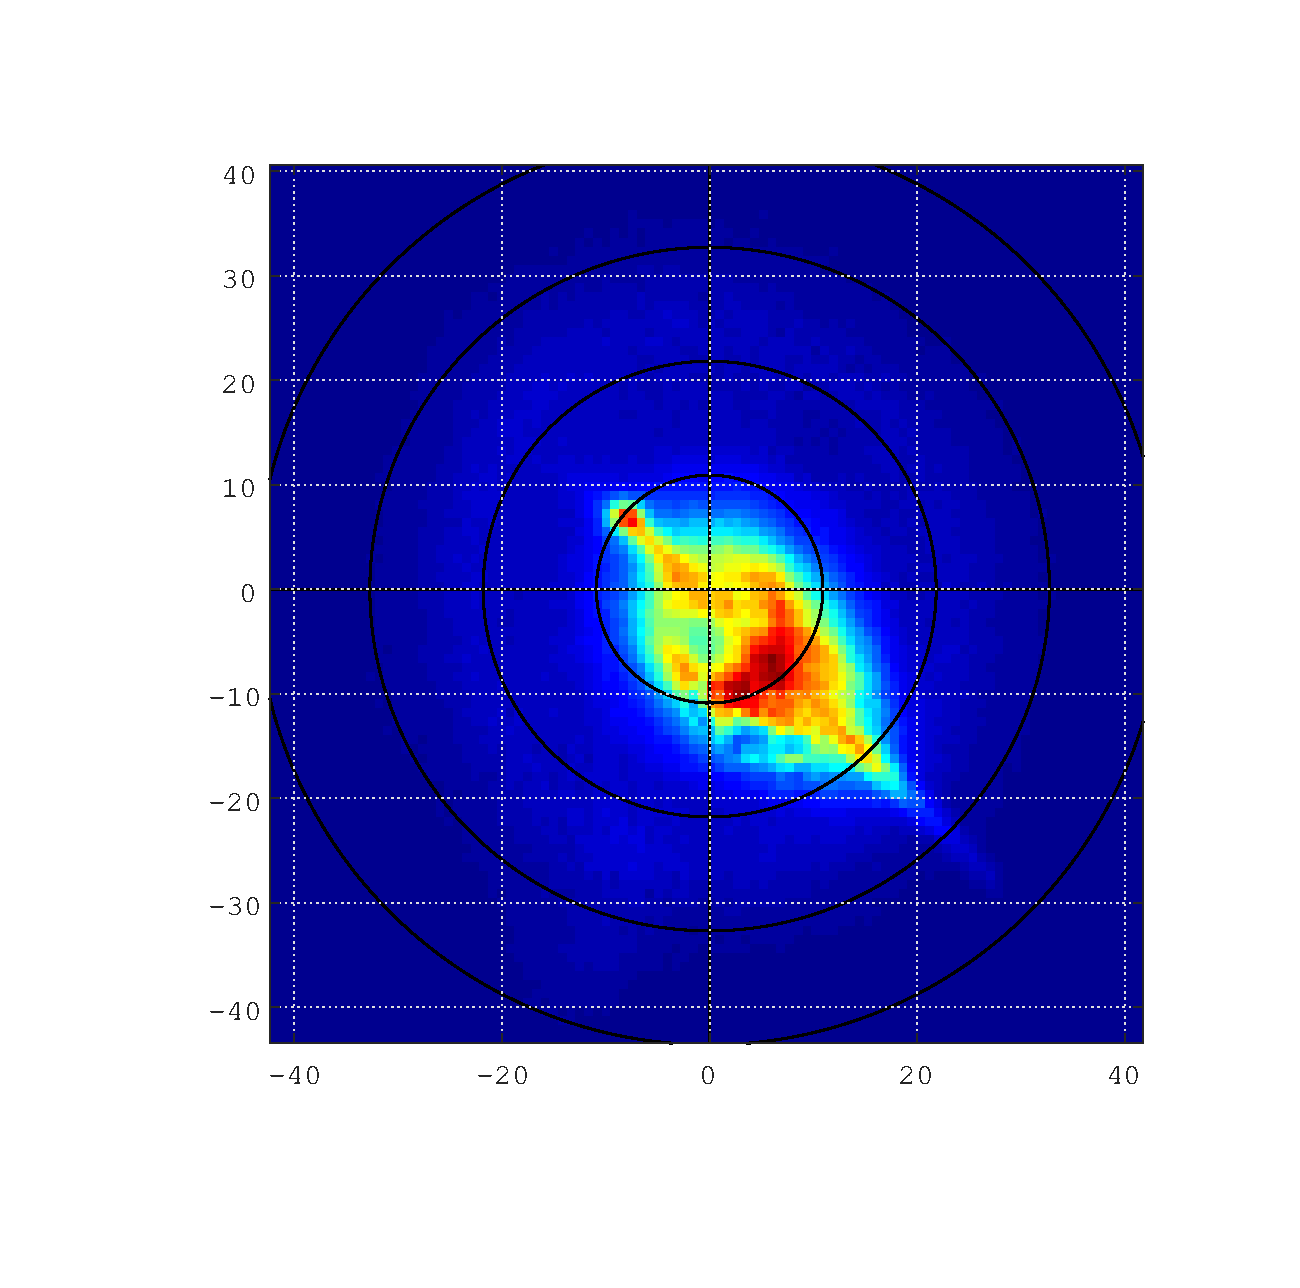
\includegraphics[width=1\textwidth]{Graphics/centre_calibration_after.eps}
  \captionof{figure}{Detector image of all hits after centring. Final values: dX = -0.5 mm, dY = 3mm}
\label{centre_calibration_after}
\end{minipage}
\end{figure}

\paragraph{Metadata parameters used by the detector image translation:}
.\newline
\lstset{language=MATLAB}
\begin{lstlisting}
exp_md.corr.det1.ifdo.dXdY 			= true; % Does this data need detector image translation correction?
exp_md.corr.det1.dX					= -0.5; %[mm] distance the center of detection is displaced left of the origin of the raw image; 
exp_md.corr.det1.dY					= 3; %[mm] distance the center of detection is displaced up the origin of the raw image;
\end{lstlisting}

\subsubsection{detector image rotation}
As seen in Figure \ref{centre_calibration_before}, the detector image shows a line of higher intensity towards the left lower corner of the detector. This is believed to originate from heavier clusters from the molecular beam. The detector image is rotated such, that this line is along the x-axis. 

\begin{figure}[h]
   \centering
    \centerline{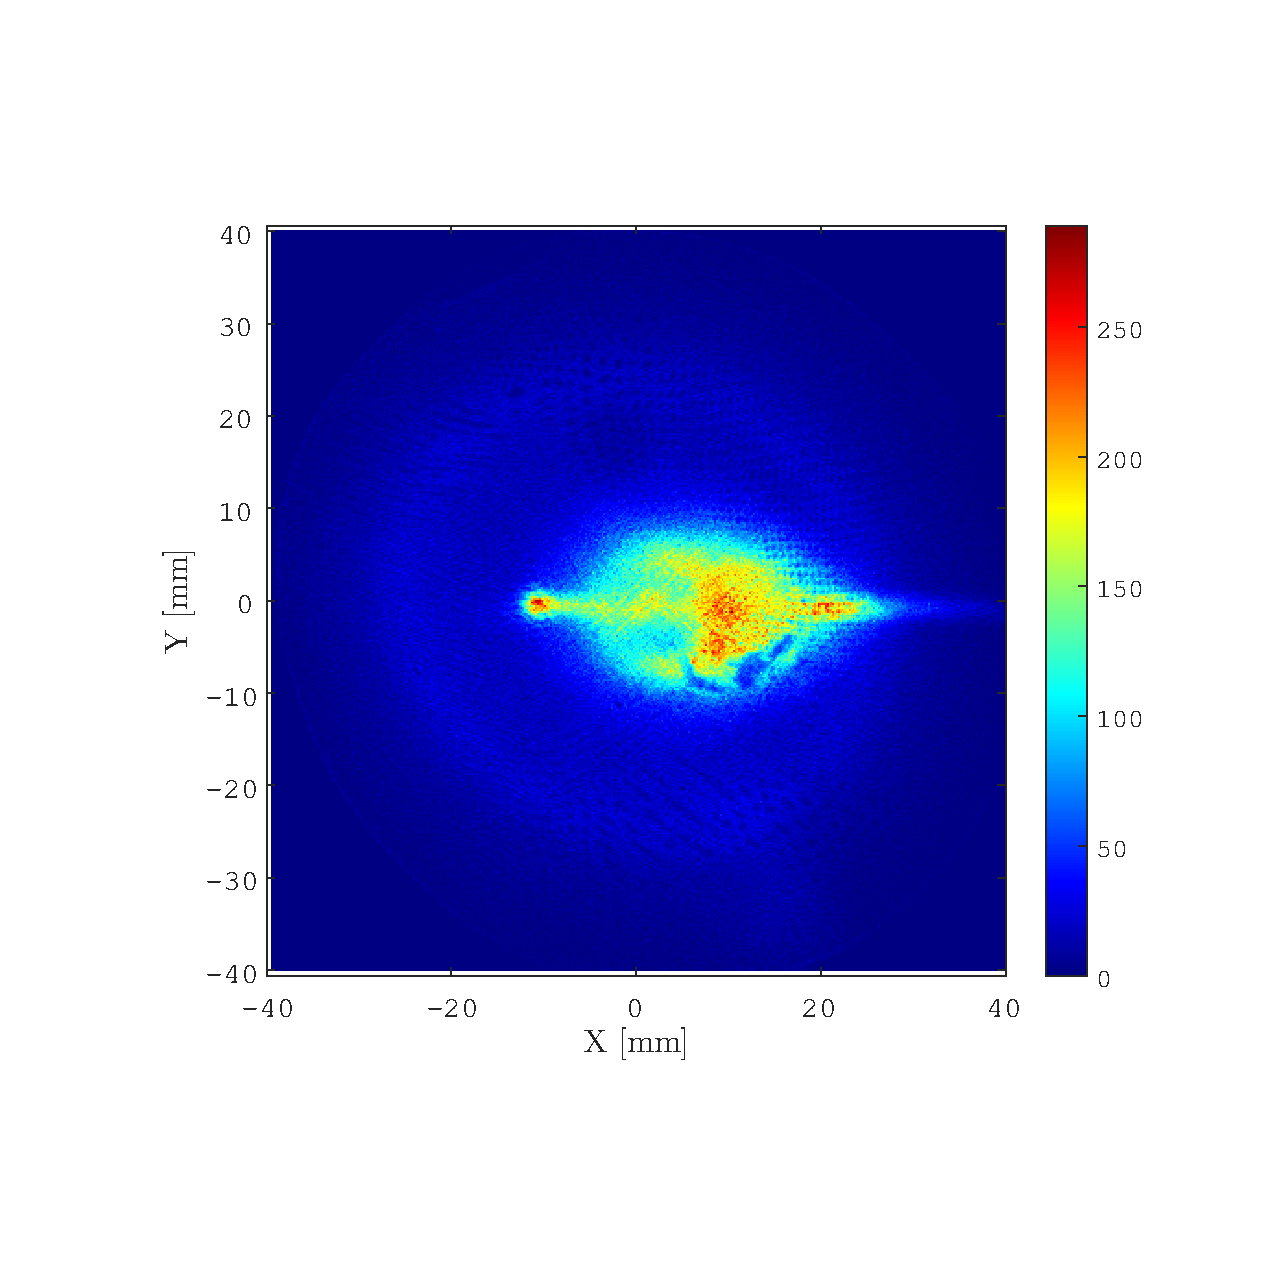
\includegraphics[width=0.5\textwidth]{Graphics/rotation_after.eps}}
\caption{The detector image rotated such that the molecular beam is aligned with the x-axis. In this case, it means an anti-clockwise rotation of 44 degrees.}
\label{Data_structure_schematic}
\end{figure}

\paragraph{Metadata parameters used by the detector image rotation:}
.\newline
\lstset{language=MATLAB}
\begin{lstlisting}
exp_md.corr.det1.ifdo.dTOF  		= true; % Does this data need detector absolute TOF correction?
exp_md.corr.det1.dTheta				= 44;   %[deg] rotation of hits around the raw image centre (anticlockwise);
\end{lstlisting}

\subsubsection{Absolute TOF translation}
The recorded time of flight can have a deviation from the actual one, due to timing differences. These can for instance originate from different signal propagation times of the trigger and the detector signal.

\paragraph{Metadata parameters used by the absolute TOF translation:}
.\newline
\lstset{language=MATLAB}
\begin{lstlisting}
exp_md.corr.det1.ifdo.dTheta 		= true; % Does this data need detector image rotation correction?
exp_md.corr.det1.dTOF 			 	= -16.7; % [ns] The difference between signal propagation times of trigger and hits
\end{lstlisting}

\subsubsection{TOF deviation due to detector-drift tube voltage mismatch}

If the MCP front voltage is not kept at the same voltage as the drift tube, the local field in front of the detector will not be uniform, but curved instead (see Figure \ref{detector_abberation_ray_traces}. This will cause a distortion in the actual TOF, compared to the one predicted assuming a pure drift of the ions in the drift tube. The Time Of Flight will decrease if the detector front is kept at a higher absolute voltage. Moreover, this influence is dependent on the position on the detector. If the ion approaches the detector out of center, the decelleration is later, because the field inhomogenity starts later. Therefore, a correction dependent on radius is needed. First, the correction in TOF is presented, and consequently the correction in splat radius is discussed.

\begin{figure}[h]
   \centering
    \centerline{\includegraphics[width=0.5\textwidth]{Graphics/detector_abberation_ray_traces.png}}
\caption{Ray traces showing the non-uniform field around the detector due to the voltage mismatch. In this case, the drift tube is kept at -4 kV and the detector front at -2 kV}
\label{detector_abberation_ray_traces}
\end{figure}


\paragraph{Step 1: Zero kinetic energy TOF correction}

The first step is to adjust the TOF of all particles such that the particles with no kinetic energy (ending up in the centre) have the right time of flight. The correction is done by shifting the measured TOF with an aomunt that is determined from analytical prediction and SIMION simulations. The driving force for the deviation is the difference between the detector and the drift tube voltage. Therefore, we investigate the TOF difference as a function of this difference. We define the following unit-less variables:

\begin{align}
V_{nd} 		= \frac{V_{det} - V_{drift}}{V_{created} - V_{drift}} \\
TOF_{nd} 	= \frac{TOF - TOF_{noKE}}{TOF_{noKE}}
\end{align}
in which $V_{det}$ is the detector front voltage, $V_{drift}$ is the drift tube voltage and $V_{created}$ is the electrostatic potential in which the particle is created. $TOF$ is the measured time of flight and $TOF_{noKE}$ the time of flight of a zero-energy particle, without the lens abberation. This is the variable we are after. Note that if $V_{det} = V_{created}$ ($V_{nd} = 1$), the charge particle has no net gain in energy from source to detector. Therefore, around this voltage configuration the TOF abberation is expected to change considerably. Indeed, a steep asymptote-like behaviour is observed around this point in Figure \ref{dTOF_vs_dV}. 

The variables $V_{nd}$ and $TOF_{nd}$ have a fixed relation, independent of:
\begin{itemize}
\item absolute drift tube voltage
\item mass of particle under study
\item field strength in the source region
\end{itemize}

This relation is approximated by a fitted curve. Since the curve shown in Figure \ref{dTOF_vs_dV} shows behaviour similar to the natural logarithm function, a following polynomial fitting curve is used:

\begin{equation}
TOF_{nd} 	= p_2 \cdot \left(ln(1 -V_{nd}) \right)^2 + p_1 \cdot \left(ln(1 - V_{nd}) \right)
\end{equation}
with $p_i$ the fitting parameters. For the shown example, $p_2 = -1.230e-2$, $p_1 = -1.193e-3$.

\begin{figure}[h]
   \centering
    \centerline{\includegraphics[width=0.9\textwidth]{Graphics/dTOF_vs_dV_dT_-8_-4_-2kV.eps}}
\caption{The Voltage and TOF dimensionless variables plotted for different absolute drift tube voltages. Similar behaviour for varying particle masses, and extraction field strengths.}
\label{dTOF_vs_dV}
\end{figure}

\paragraph{Step 2: TOF correction as a function of radius}
The TOF correction described in step 1 is applied to all hits. However, hits with different splat radii see a different voltage profile along its trajectory, and will therefore be affected differently. We define the following nondimensional variables:

\begin{align}
R_{nd} 		= \frac{R}{R_{det}}\\
TOF_{nd} 	= \frac{TOF_{noKE} - TOF_{corr}}{TOF_{corr}}
\end{align}

in which $R$ is the splat radius, $R_{det}$ the radius of the detector, $TOF_{noKE}$ the corrected time of flight for zero-kinetic energy particles and ${TOF_{corr}}$ the corrected time of flight including the radial correction. This is the variable we are after. The difference in time of flight appears to increase in a quadratic fashion, see Figure \ref{dTOF_dR_nd}. This dependency is, again, independent of absolute voltages, particle masses and interaction field strength. 

\begin{figure}[h]
   \centering
    \centerline{\includegraphics[width=0.9\textwidth]{Graphics/dTOF_dR_nd.eps}}
\caption{The difference in TOF due to a difference in field distortion at different radii. In this example the curve is fitted with $p_2 = -6.32e-3$ and $p_3 = -1.88e-3$. }
\label{dTOF_dR_nd}
\end{figure}

The curve is fitted with the following polynomial:
\begin{equation}
\frac{TOF_{nd}}{V_{nd}} 	= p_2 \cdot \left(R_{nd}) \right)^2 + p_3 \cdot \left(R_{nd}) \right)^3
\end{equation}

The shown correction is validated by comparing it with the theoretical mass to charger conversion factor and the one with and without the correction. The theoretical value is around 965. Without correction, a factor of about 971.7 is found. After correcting, this factor is around 965, so very close to the theoretical value.

\paragraph{Step 3: Correction of splat radius linearity}
Now that the time of flight is corrected for all hits, the splat radius will be corrected. The splat radius is expected to increase linearly with the transverse momentum vector magnitude, and this step corrects the splat radius such that it does. The example trajectories in Figure \ref{detector_abberation_ray_traces} show an outward curve, implicating that the corrected splat radius needs to be smaller than the registered one. This behaviour will be the other way around when the voltage difference is flipped. Therefore, the behaviour is expected to be related to the voltage difference. We assume a inverse proportional relation:

\begin{equation}
\frac{R - R_{corr}}{R_{det}} =  p_1 \cdot V_{nd} \cdot R_{nd}
\end{equation}
in which $R$ is the measured radius and $R_{corr}$ the corrected value. In the example shown in figure \ref{Radius_correction_det_abb}, $p_1 = 0.278$.


\begin{figure}[h]
   \centering
    \centerline{\includegraphics[width=0.6\textwidth]{Graphics/Radius_correction_det_abb.eps}}
\caption{The splat radius correction needed, as a funtion of detector front voltage.}
\label{Radius_correction_det_abb}
\end{figure}

\begin{figure}[h]
   \centering
    \centerline{\includegraphics[width=0.8\textwidth]{Graphics/SIMION_det_corr_both.eps}}
\caption{The momenta histograms ($\vec{p_x}$, $\vec{p_z}$) and KER histogram without detector abberation correction (top) and with correction (bottom). SIMION simulations, m = 18 a.m.u, singly charged, KE = 3 eV, $\sigma$(KE) = 0.1eV, 50000 particles. Drift tube @ -4kV, detector front @ -2kV.}
\label{Radius_correction_det_abb}
\end{figure}

\paragraph{Metadata parameters used by the detector abberation correction}
.\newline
\lstset{language=MATLAB}
\begin{lstlisting}
exp_md.corr.det1.ifdo.detectorabb	= true; % Does this data need detector-induced abberation correction?
exp_md.spec.volt			= 0;     %[V] used voltages on electrodes;
exp_md.det.det1.Front_Voltage  	= -2000; % [V] Detector front potential.
exp_md.det.det1.max_radius 		= 40 ; %[mm] Radius of the detector
exp_md.corr.det1.detectorabb.TOF_noKE.p_i	= [-111 -1242 0]*1e-5; % The polynomial fit parameters for the TOF correction, making all zero-kinetic energy TOF's equal to the one without abberation.
exp_md.corr.det1.detectorabb.TOF_R.p_i		= [-1.88  -6.32 0  0]*1e-3;% The polynomial fit parameters for the radial TOF correction
exp_md.corr.det1.detectorabb.dR.p_i			= [0.28 0]% The polynomial fit parameters for the radial correction
\end{lstlisting}

\paragraph{TOF lens abberation correction}
The TOF of a charged particle is not independent of its transversal momentum. In other words; the TOF of a particle with zero kinetic energy is different from the TOF of a particle that has an initial momentum perpendicular to the spectrometer axis. This is a direct consequence of the use of non-uniform fields (lensing). Correcting for this abberation is necessary for the KER determination. We choose a similar approach as presented before, by choosing non-dimensional parameters. Note that this correction is very similar to the one described in `step 1' and '`step 2' of the detector abberation correction.


\paragraph{Step 1: Zero kinetic energy TOF correction}
We define the following dimensionless variables:

\begin{align}
V_{nd} 		= \frac{V_{lens} - V_{drift}}{V_{created} - V_{drift}} \\
TOF_{nd} 	= \frac{TOF - TOF_{noKE}}{TOF_{noKE}} \\
\end{align}
in which $V_{lens}$ is the lens voltage, $V_{drift}$ is the drift tube voltage and $V_{created}$ is the electrostatic potential in which the particle is created. $TOF$ is the measured time of flight and $TOF_{noKE}$ the time of flight of a zero-energy particle, without the lens abberation. This is the variable we are after. 

\begin{figure}[h]
   \centering
    \centerline{\includegraphics[width=0.8\textwidth]{Graphics/lens_dTOF_vs_dV_dT_-8_-4_-2kV.eps}}
\caption{The Voltage and TOF dimensionless variables plotted for different absolute drift tube voltages. The fit shown uses the parameters $p_3 = 1.13e-3$, $p_2 = 3.48e-3$ $p_4 = 10.4 e-3$}
\label{Radius_correction_det_abb}
\end{figure}

The variables $V_{nd}$ and $TOF_{nd}$ have a fixed relation, independent of:
\begin{itemize}
\item absolute drift tube voltage
\item mass of particle under study
\item field strength in the source region
\end{itemize}

The relation is fitted by a mean-square polynomial fit:
\begin{equation}
TOF_{nd}	= p_3 \cdot \left(V_{nd}) \right)^3 + p_2 \cdot \left(V_{nd}) \right)^2 + p_1 \cdot \left(V_{nd}) \right)^1
\end{equation}

\paragraph{Step 2: TOF correction as a function of radius}
Not implemented yet

\paragraph{Step 3: Correction of splat radius linearity}
The linearity of the radial splat with increasing velocity gets a bit lost with the use of the lens. The following dimensionless variables:

\begin{align}
V_{nd} 		= \frac{V_{lens} - V_{drift}}{V_{created} - V_{drift}} \\
R_{ratio}	= \frac{R_{corr}}{R}
\end{align}

The fit is shown in Figure \ref{dR_correction_fit}.

\begin{figure}[h]
   \centering
    \centerline{\includegraphics[width=0.8\textwidth]{Graphics/dR_correction_fit.eps}}
\caption{The linearity correction due to the lens abberation.}
\label{dR_correction_fit}
\end{figure}

\begin{figure}[h]
   \centering
    \centerline{\includegraphics[width=0.8\textwidth]{Graphics/SIMION_lens_corr_both.eps}}
\caption{The momenta histograms ($\vec{p_x}$, $\vec{p_z}$) and KER histogram without lens abberation correction (top) and with correction (bottom). SIMION simulations, m = 18 a.m.u, singly charged, KE = 3 eV, $\sigma$(KE) = 0.1eV, 50000 particles. Drift tube @ -4kV, lens @ -3270V.}
\label{SIMION_lens_corr_both}
\end{figure}

It is tested and verified that the corrections can be applied to the same data, so the detector correction first, followed by the lens abberation correction.

\subsubsection{Non-circular correction}
It can be the case that a spectrometer shows non-circular patterns in the data, where a purely circular pattern is expected from physical principles. There is a routine developed that detects a maximum along the angle in a 2D histogram with the angle (X) and another physical property (Y). 

An example of such a conversion can be found in Figure \ref{R_circle_corr}, the result of a measurement at the EPICEA spectrometer, at the toroidal energy analyzers. The routine calculates a maximum intensity within specified radial regions, called the 'Region Of Interest' (ROI), see the black encircled boxes in Figure \ref{R_circle_corr} left. The maximum-finding procedure uses median filters to the histogram in both angle (phi) and physical quantity (in this case, R) direction, to obtain a maximum line that is smoother and does not get distorted by outliers.

At zero radius, the data points will never be shifted. It is thus important to first calibrate the detection centre correctly. To prevent interpolation out of range, the relative shift at the radial peak value is applied at a radius twice the radial peak value. 

The radial values are shifted in a linear interpolation between the known points from the calibration. The interpolation is thus only applied in radial direction. 

\begin{figure}[h!]
         \centering
    	 \centerline{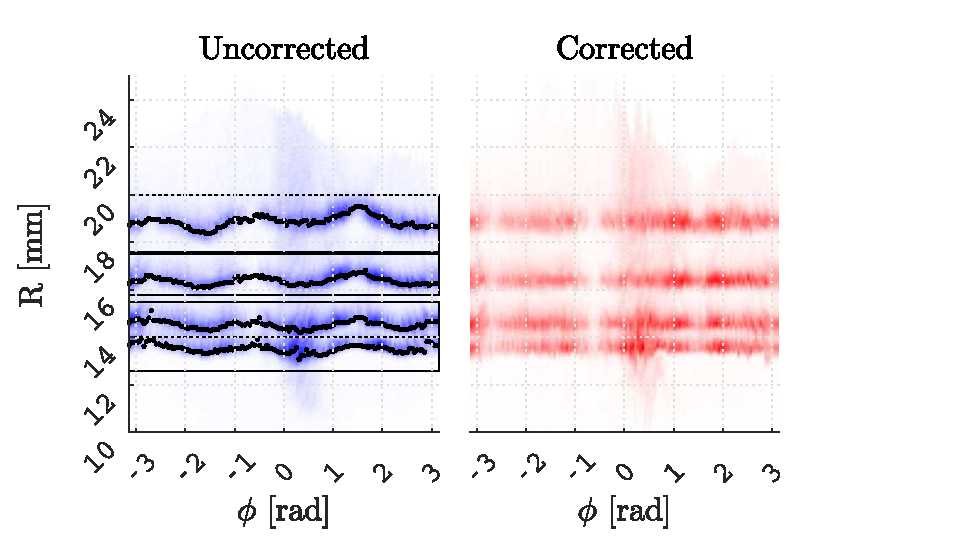
\includegraphics[width=0.8\textwidth]{Graphics/ESCA_R_circle_corr.eps}}
\caption{Left: Histogram showing the angle-dependent electron radial position from a toroidal energy analyzer. In this analyzer, the radial position is converted to electron kinetic energy. The non-circular abberation causes the oscillatory pattern, making the radius to electron energy conversion ambiguous. Right: the corrected electron radial position, showing a horizontal stripe pattern, so that a radial position corresponds to a electron energy. The location of the suspected cause of the instability (physical holders in the spectrometer) are indicated in the right plot. Data: photolines upon C1s ionization of trifluoroacetate (`ESCA molecule') at 411 eV photon energy.}
\label{R_circle_corr}
\end{figure}



\newpage
\subsection{convert}

\subsubsection{TOF $\rightarrow m/q$}

\subsubsection{Signal labeling - single coincidence}
By repeating a certain filtering operation onto the same signal, but with changing filtering conditions, an array with a set of labels can be written. In this example we only discuss the labeling of TOF hits to `Mass-over-charge' values.\\
For example: A TOF between 950 and 1000 ns is understood as hits that originate from a mass2charge value of 1, and a TOF between 4080 and 4120 ns is understood to come form a mass2charge value of 18. A label array contains expected mass2charge values at the corresponding hits that are identified to belong to that mass2charge. There will be broadening of any TOF peak, but we can label all peaks around a certain expectation value. This broadening is called the `search radius' in this code. Signal labeling can be done for an array of expected mass2charge values, resulting in an array with a label for every hit. No identification of a hit will result in NaN. \\
The definition of the conversion factor is as follows:
\begin{equation}
TOF = t_0 + factor*\sqrt(M2Q)
\end{equation}
Note that the $t_0$ is a correction value and is already substracted from the measured TOF in the `correct' section.

\subsubsection{Signal labeling - double coincidence}
In the case of a double coincidence event (two hits registered on one detector in one event), the filtering conditions of the measurement can be fine tuned. In this software, two methods are available;  the `circle', in which a certain maximum distance between the nominal m2q-values are approved. The other method, `line', approves all hits along a diagonal line representing a constant TOF. 

\paragraph{circle} In a two-dimensional histogram of two mass-over-charge values, only hits within a certain circle are approved. This can be of use in the case of cluster measurements, where the momenta of two cations are not necessarily related. See Figure \ref{labeling_C2} for an example.

\begin{figure}[H]
   \centering
    \centerline{\includegraphics[width=0.9\textwidth]{Graphics/M2Q_labeling_C2_circle_example.eps}}
\caption{example of a `circle' filter around the nominal mass-over-charge values. Circle radius of 0.25 mass-over-charge units. Example of water-ammonia clusters.}
\label{labeling_C2}
\end{figure}

\paragraph{line} 
In a two-dimensional histogram of two mass-over-charge values, only hits with a TOF-sum that is close to the nominal one, is approved. This is useful when the detection is complete, and can therefore be regarded to have opposite momenta in z-direction. 

\begin{figure}[H]
   \centering
    \centerline{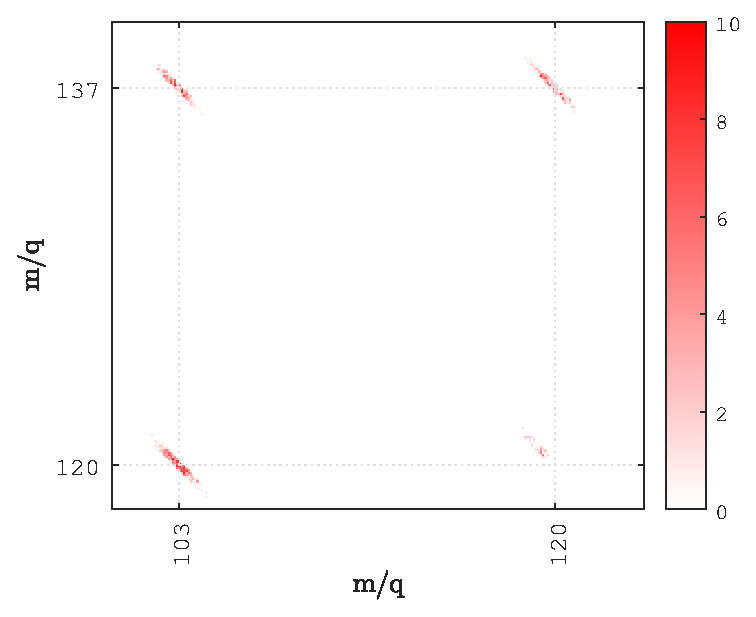
\includegraphics[width=0.5\textwidth]{Graphics/M2Q_labeling_C2_line_example.eps}}
\caption{Example of a `line' filter around the nominal mass-over-charge values. Circle radius of 0.2 mass-over-charge units. Example of ammonia clusters.}
\label{labeling_C2}
\end{figure}

\subsubsection{Branching ratio's}
The braching ratio is defined here as the relative number of hits registered for a label, or a set of labels. In the presented example, branching ratio's of mass-over-charge labels are shown. \\

\paragraph{Single-label Branching ratio's}

The Branching ratio of single labels simply counts the number of hits are categorized into a certain label. As an example, figure \ref{BR_1D} shows the number of occurences of particles recognized as having certain mass-2-charge values. Note that these labels can be defined independently from the events.

\begin{figure}[H]
   \centering
    \centerline{\includegraphics[width=0.9\textwidth]{Graphics/BR_1D.eps}}
\caption{Example of a branching ratio plot. This example: NH$_3$ clusters, filename called `20091115\_NH3\_n17'}
\label{BR_2D}
\end{figure}

\paragraph{Double-label Branching ratio's}
If multiple hits are registered in one event, the possible combinations of labels can be studied. If there are $n$ labels registered, then $n^2$ combinations of labels can be registered. The double-label branching ratio is the histogram of these combinations, with a differentiation between label A registered before label B and label A registered after label B. In Figure \ref{BR_2D}, an example of such two-label branching ratio plot is shown. It shows which mass-to-charge particle is registered in combination with another. All the first labels registered have smaller mass-to-charge values, because the labels are based on the TOF values of the hits.

\begin{figure}[H]
   \centering
    \centerline{\includegraphics[width=0.6\textwidth]{Graphics/BR_2D.eps}}
\caption{Example of a branching ratio plot for double labels (double coincidence). The color of the dots represents the branching ratio of that set of labels. This example: NH$_3$ clusters, filename called `20091115\_NH3\_n17'}
\label{BR_1D}
\end{figure}

\subsubsection{Momentum}

TODO: describe the Maxwell-Boltzmann distribution assumption!
\begin{align}
V_{avg} = \sqrt{\frac{\gamma}{\gamma - 1}} \sqrt{\frac{2 R T}{W}}
\end{align}

\begin{figure}[H]
  \centering
  \vspace{0 cm}
  \def\svgwidth{200pt}
  \centerline{\input{Graphics/momentum_subtraction.pdf_tex}}
  \caption{Schematic of the Momentum along the molecular beam, $\vec{p}_{0}$}
\end{figure}


In the case of momentum imaging, the splat radius on the detector gives info about the momentum in the transverse direction (here called the $x$ and $y$-direction. In the first approximation, the splat radius increases linearly with the momentum in each direction.\\
The momentum in the detector axis can be inferred from the difference between the actual and the zero kinetic energy time of flight of the particle.\\
The sample, leaving the molecular beam, has a low mean velocity in directions perpendicular to the beam. However, the velocity distribution in the molecular beam direction has a higher mean value. 
This will show up in the data as a spatial shift of the detection centre at higher Times Of Flight. 

\begin{figure}[H]
   \centering
    \centerline{\includegraphics[width=0.9\textwidth]{Graphics/p_0_subtraction_before.eps}}
\caption{Radius vs TOF, showing the shift of hits outward. The line is plotted with a prediction from a Maxwell-Boltzmann expectation value of the velocity ($T_{sample} = $ 38 [deg]). Example: Ammonia/Water clusters at 450 eV. (20130903\_008.dlt)}
\end{figure}

The momentum in x and y-direction (parallel to detector plane) can be calculated from the simple equation $s = v \cdot t$:

\begin{equation}
\vec{p}_{x, y} =  \frac{m \cdot X}{TOF}
\end{equation}

The momentum in z-direction (perpendicular to detector plane) is calculated as:

\begin{equation}
\vec{p}_{z} = q \cdot E_{ER} \cdot \Delta TOF
\label{p_z_2_TOF}
\end{equation}
where $\Delta TOF$ is defined as the difference between the zero-momentum Time Of Flight and the actual Time Of Flight. $E_{IR}$ is the electric field strength in the interaction region.
We define two different momenta: the momentum of the sample before the photon interaction takes place ($\vec{p_0}$), and the momentum after the interaction has taken place ($\vec{p}$). Note that the kinetic energy released following photon interaction should calculate with the difference of these two vectors:

\begin{equation}
KE = KE(\vec{p} - \vec{p_0}) = \frac{1}{2 m} \cdot |{\vec{p} - \vec{p_0}}|^2
\end{equation}

\paragraph{$\vec{p_0}$ determination}
The zero-time momentum $\vec{p_0}$ is determined from the difference in the mean value of the X, Y and TOF and their zero-momentum expectation values. These zero-momentum expectation values are 0 for X and Y (assuming a proper correction of the detection centre, see signal correction), and given by the expected mass over charge labels for the TOF signal. The averaging is done over all hits belonging to one label. For instance, a label could be an OH$^+$ fragment. 

\paragraph{$\vec{p}$ determination}
The final momentum $\vec{p}$ is determined by the difference in measured detector position and the zero-momentum expectation values. Note that this value can be different for every hit, whereas $\vec{p_0}$ is determined for every label (containing multiple hits). 

\begin{figure}[H]
   \centering
    \centerline{\includegraphics[width=0.4\textwidth]{Graphics/pxpy_hist.eps}}
\caption{The total momentum ($p$) and the total minus the zero-time momentum ($p - p_0$) compared. In this example, the molecular beam is directed along the x-axis, coming from the left. It is seen that the mean value of total momentum shifts along the molecular beam axis, which is  
Example of pure NH3 clusters for cluster sizes of n = 1, 5, 10 in (NH$_3$)$_n^+$H}
\end{figure}

\subsubsection{Kinetic Energy Release}

If all three momentum components of a particle can be determined, the kinetic energy of that particle can be calculated:

\begin{equation}
KE = \frac{1}{2 m} \cdot \left(p_x^2 + p_y^2 + p_z^2 \right)
\end{equation}

\begin{figure}[H]
    \centering
        {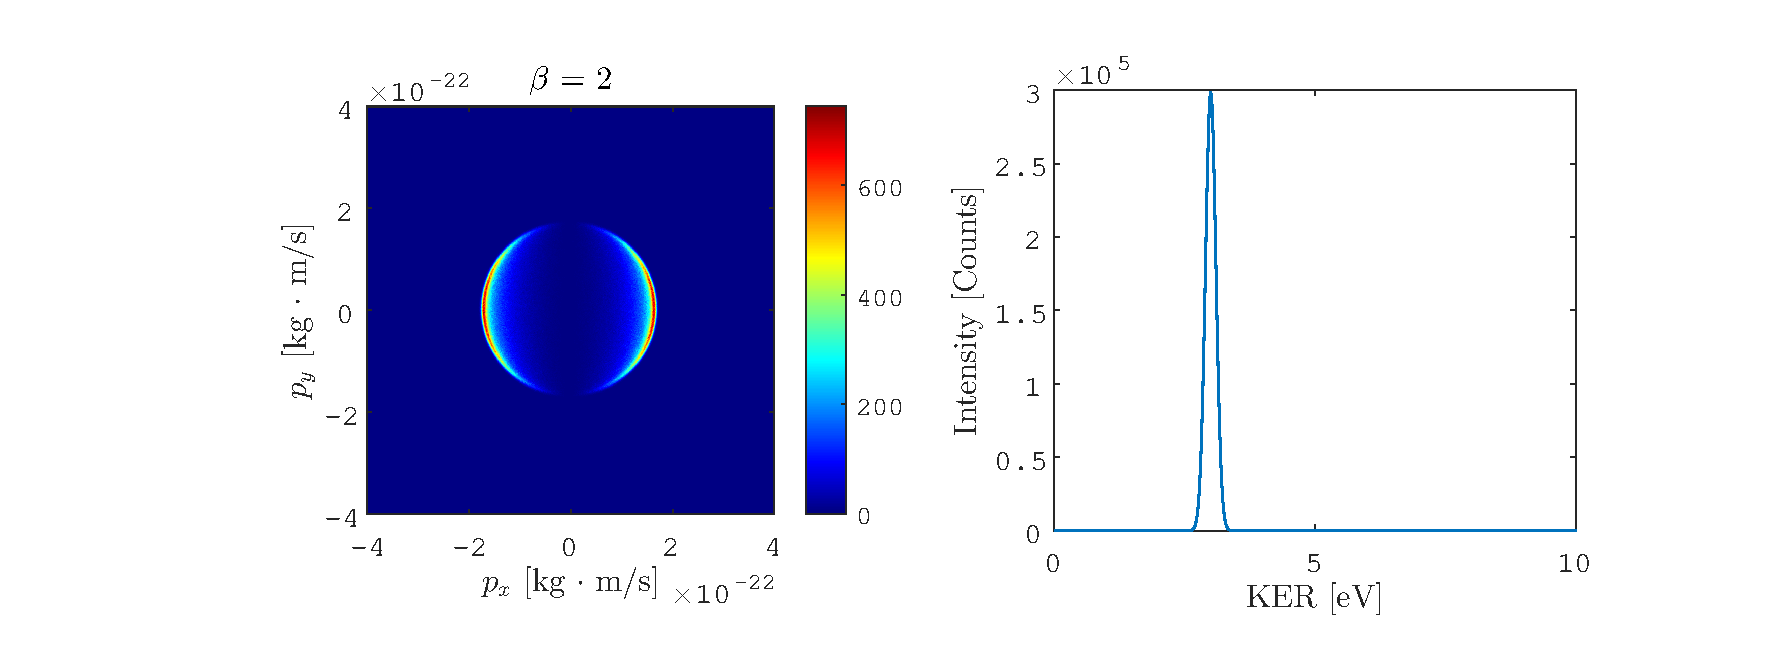
\includegraphics[width=0.7\textwidth]{Graphics/KER_dummy_data_beta_2.eps}
    }\\
        {\includegraphics[width=0.7\textwidth]{Graphics/KER_dummy_data_beta_0.eps}
    }\\
        {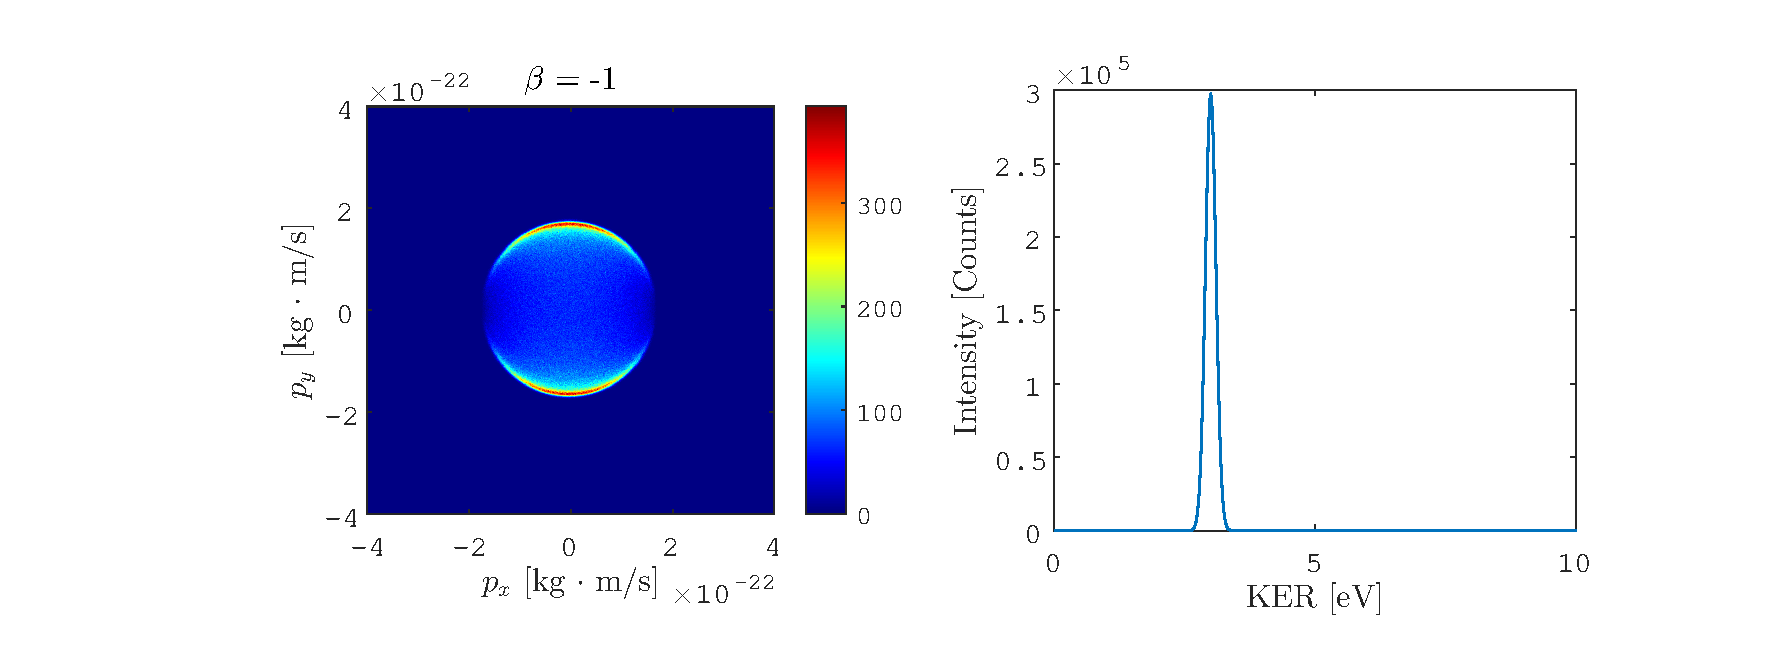
\includegraphics[width=0.7\textwidth]{Graphics/KER_dummy_data_beta_-1.eps}
    }
    \caption{The kinetic energy release does not change for different angular distributions ($\beta$-values). Fake data created with the parameters: m = 18 a.m.u, singly charged, KE = 3 eV, $\sigma$(KE) = 0.1eV. Polarization is horizontal in the screen.}
    \label{TS}
\end{figure}

\subsubsection{Mutual momentum angle}
the angle between two three-dimensional momentum vectors is measured by the shortest great circle path between them, which means that it must lie between 0 and pi radians.

\begin{figure}[H]
  \centering
  \vspace{0 cm}
  \def\svgwidth{200pt}
  \centerline{\input{Graphics/mutual_angles.pdf_tex}}
  \caption{The shortest great circle path between two three-dimensional momentum vectors is called $\theta$.}
\end{figure}

\subsubsection{Asymmetry parameter $\beta$}
TODO

\subsubsection{Interaction point}
In the event of complete ion detection of an initially cold sample, the initial source point position can be calculated. If we assume the sum of all momenta to be equal to zero:

\begin{equation}
p_{res, x} = \sum_i {\frac{m_i \cdot (X_i - X_{0})}{TOF_i}} = 0
\end{equation}
where $i$ is the amount of hits registered in one event. Form this equation, we can extract information on the creation point of the mother particle. This equation can in general be solved for any $i$:

\begin{equation}
X_0 = \frac{ \sum_i {\tfrac{m_i}{TOF_i} X_i} }
						{ \sum_i {\tfrac{m_i}{TOF_i} } }
\label{X_CM}
\end{equation}

In the case of a single-hit event, equation \ref{X_CM} simplifies to $X_0 = X_1$, so in these approximations, the registration of mother ions images the source volume. Equation \ref{X_CM} is valid for X and Y. \\
For the Z-direction (TOF), we identify three contributions to the measured TOF:

\begin{align}
\underbrace{TOF_{exp}} _\textrm{measured TOF} &= 
\underbrace{TOF  (Z = 0, p = 0)}_\textrm{nominal TOF, or $TOF_0$} + 
\underbrace{\Delta TOF (Z = 0, p = p_z)}_\textrm{p-induced TOF shift} +
\underbrace{\Delta TOF (Z = Z_0, p = 0)}_\textrm{Z-induced TOF shift}
\end{align}

The TOF difference induced by the momentum can be written as (see Eq. \ref{p_z_2_TOF}):

\begin{equation}
\Delta TOF (Z = 0, p = p_z) = \frac{p_z}{q \cdot E_{ER}}
\end{equation}

The TOF difference induced by the Z-displacement is the relation under study here. Note that this number is minimized by the Wiley-McLaren condition, so this calculation can be error-prone when exact Wiley-McLaren conditions are met. We assume the linear condition:

\begin{equation}
\Delta TOF (Z = Z_0, p = 0) = \frac{C \cdot Z_0}{\sqrt{m/q}}
\end{equation}

In case of Wiley McLaren conditions met, C = 0 (see Figure \ref{dZ_vs_dTOF_Laksman}), and the presented treatment cannot be used.

\begin{figure}[H]
   \centering
    \centerline{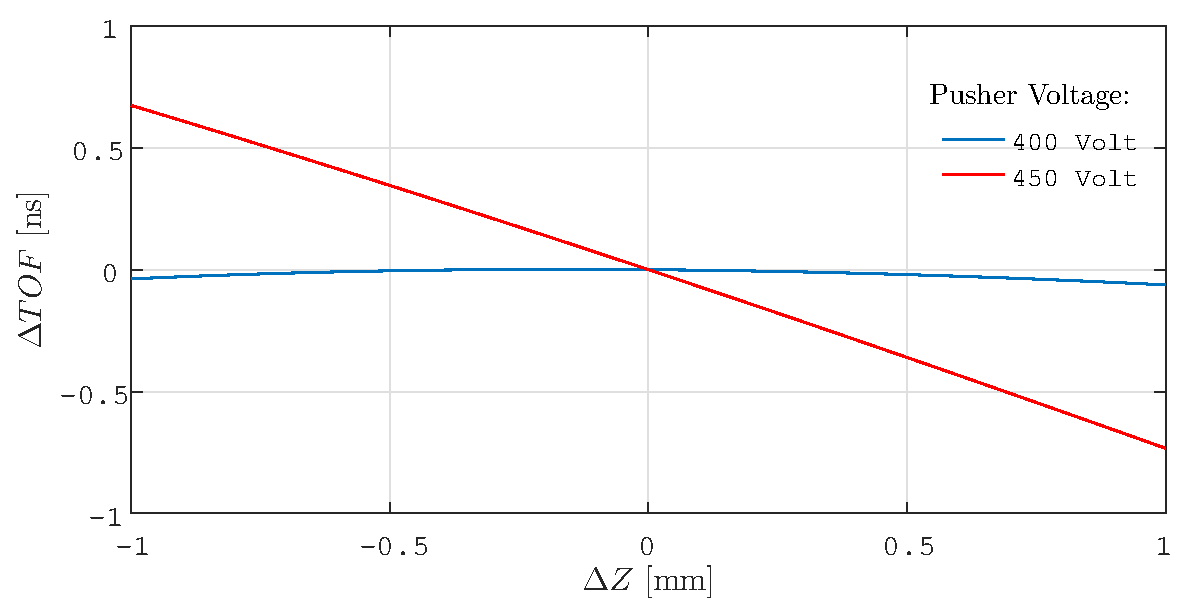
\includegraphics[width=0.8\textwidth]{Graphics/dZ_vs_dTOF_Laksman.eps}}
\caption{Example of how the change in dZ affects the effective (TOF Laksman). Two examples of ion `pusher' voltages are shown. The 400 Volt example meets the Wiley-McLaren condition, but the 450 Volt example does not. In this treatment, the correlation is assumed linear. $m/q = 1$, Drift tube voltage = -4kV.}
\label{dZ_vs_dTOF_Laksman}
\end{figure}

With this description of the TOF, we can use momentum conservation:

\begin{align}
p_{res, z} = \sum_i{p_{z, i}} = E_{ER} \cdot \sum_i{\left( TOF_{exp, i} - TOF_0 - \tfrac{b \cdot Z_0}{\sqrt{m/q_i}} \right) \cdot q_i} = 0\\
\sum_i{\left( TOF_{exp, i} - TOF_0 \right) \cdot q_i} = 
\sum_i{\tfrac{b \cdot Z_0}{\sqrt{m/q_i}} \cdot q_i }
\end{align}

Note that $Z_0$ is an event property, and is thus the same for all hits in the same event. To write $Z_0$ explicitly:

\begin{equation}
Z_0 = \frac{\sum_i{\left( TOF_{exp, i} - TOF_0 \right) \cdot q_i}}
{\sum_i{b \cdot \sqrt{\tfrac{q_i^3}{m}}}}
\end{equation}

Or, more general, not assuming a linear relation between the $\Delta TOF $ and $Z_0$:
\begin{equation}
a + b \cdot Z_0 + c \cdot Z_0^2 + ... = \frac{\sum_i{\left( TOF_{exp, i} - TOF_0 \right) \cdot q_i}}
{\sum_i{\sqrt{\tfrac{q_i^3}{m}}}}
\end{equation}

This conversion is only implemented for X and Y. See `convert.source$\_$position' for the code so far.

\subsubsection{Oversight of signals}

Here, a signal is defined as something that has a value for all hits. New signals are created by correcting a raw signal or converting a corrected signal. The signals can be found in: \emph{`Experiment name'.h.`detector name'}.`signal name'. The momentum is expressed in atomic units. \footnote{($ 1 a.u. = 1.992e-24 \cdot \tfrac{kg \cdot m}{s}$)}	

\begin{tabular}{l|c|c|c|r}
Description & MATLAB name & Type & Created from & Unit\\
\hline
detector dependent 						& raw 							& input	 								& - 														&- \\
corrected X										& X\_corr						& corrected						& X (raw)		 									& mm \\
corrected Y										& Y\_corr						& corrected						& X (raw) 										& mm \\
corrected TOF									& TOF\_corr				& corrected						& TOF(raw)  									& ns \\
mass-to-charge 								& m2q 							& converted 						& TOF\_corr									& $\tfrac{a.m.u}{a.c.u.}$ \\ 
m2q labels											& m2q\_l 					& label 									& m2q												& $\tfrac{a.m.u}{a.c.u.}$ \\ 
mass labels 										& m\_l							& label 									& m2q												& a.m.u \\
zero-time momentum, $\vec{p_0}$			& p\_0		& converted 						& X, Y, TOF, m2q\_l						& a.u.\\
final momentum, $\vec{p}$		& p 									& converted 						& X, Y, TOF, m2q\_l						& a.u.\\
momentum difference, $\vec{p} - \vec{p_0}$ & dp& converted 						& X, Y, TOF, m2q\_l						& a.u.\\
Kinetic energy release 					& KER 							& converted 						& p, p\_0 											& Joule \\
\end{tabular}	



\newpage
\subsection{filter}
In this context, filtering is defined as checking whether single hits or events holds a certain quantitative condition or criterium. No data is thrown out. Thus, the output array of a filter contains boolean (values are 'true' or 'false'). An example of an input signal filter, its input and output matrix, is given in the following table.

\begin{table}
\center
\caption{Input and output array for a filter only approving input values between and including 4 to 9. ($4 \leq x \leq 9$)}
\begin{tabular}{cc}
input array 	& output array\\
\hline
3				& false\\
4				& true\\
7				& true\\
2 				& false\\
12				& false\\
8				& true\\
1 				& false\\
\end{tabular}
\end{table}

combining multiple filters can be done in a single line.
\begin{itemize}
\item \emph{filter\_array\_3  = filter\_array\_1 \&\& filter\_array\_2} if both filter conditions should hold
\item \emph{filter\_array\_3  = filter\_array\_1 \textbar\textbar filter\_array\_2} if either condition should hold.
\end{itemize}

Filtering can be done on the events and on the hits. An example of a filter on events is the filtering of all double coincidence events. An example for hits is a TOF that filters out a certain chemical mass. When a set of hits is filtered, the corresponding hits can be identified and thus a event-based filter array can be built. This can be done with function XXXX. This can be needed when a certain condition is imposed on one detector, and the user wants to visualize the remaining events on another detector.

The filtering arrays are stored under the name \emph{filter\_h\_}*name* for events, and \emph{filter\_h\_}*det\_name* \_ *name* for hits. For the hit filter arrays, the detector name needs to be specified, since hits among different detectors need not be correlated. 


\begin{figure}[h]
   \centering
    \centerline{\includegraphics[width=0.9\textwidth]{Graphics/Filter_event2hit.pdf}}
\caption{The translation of an example event filter to a hit filter.}
\label{Data_structure_schematic}
\end{figure}

\begin{figure}[h]
   \centering
    \centerline{\includegraphics[width=0.9\textwidth]{Graphics/Filter_hit2event.pdf}}
\caption{The translation of an example hit filter to an event filter.}
\label{Data_structure_schematic}
\end{figure}


\newpage
\subsection{plot}
TODO: The available plot functions and a few examples of signals plotted.

\subsubsection{Mass to charge}

\begin{figure}[h]
   \centering
    \centerline{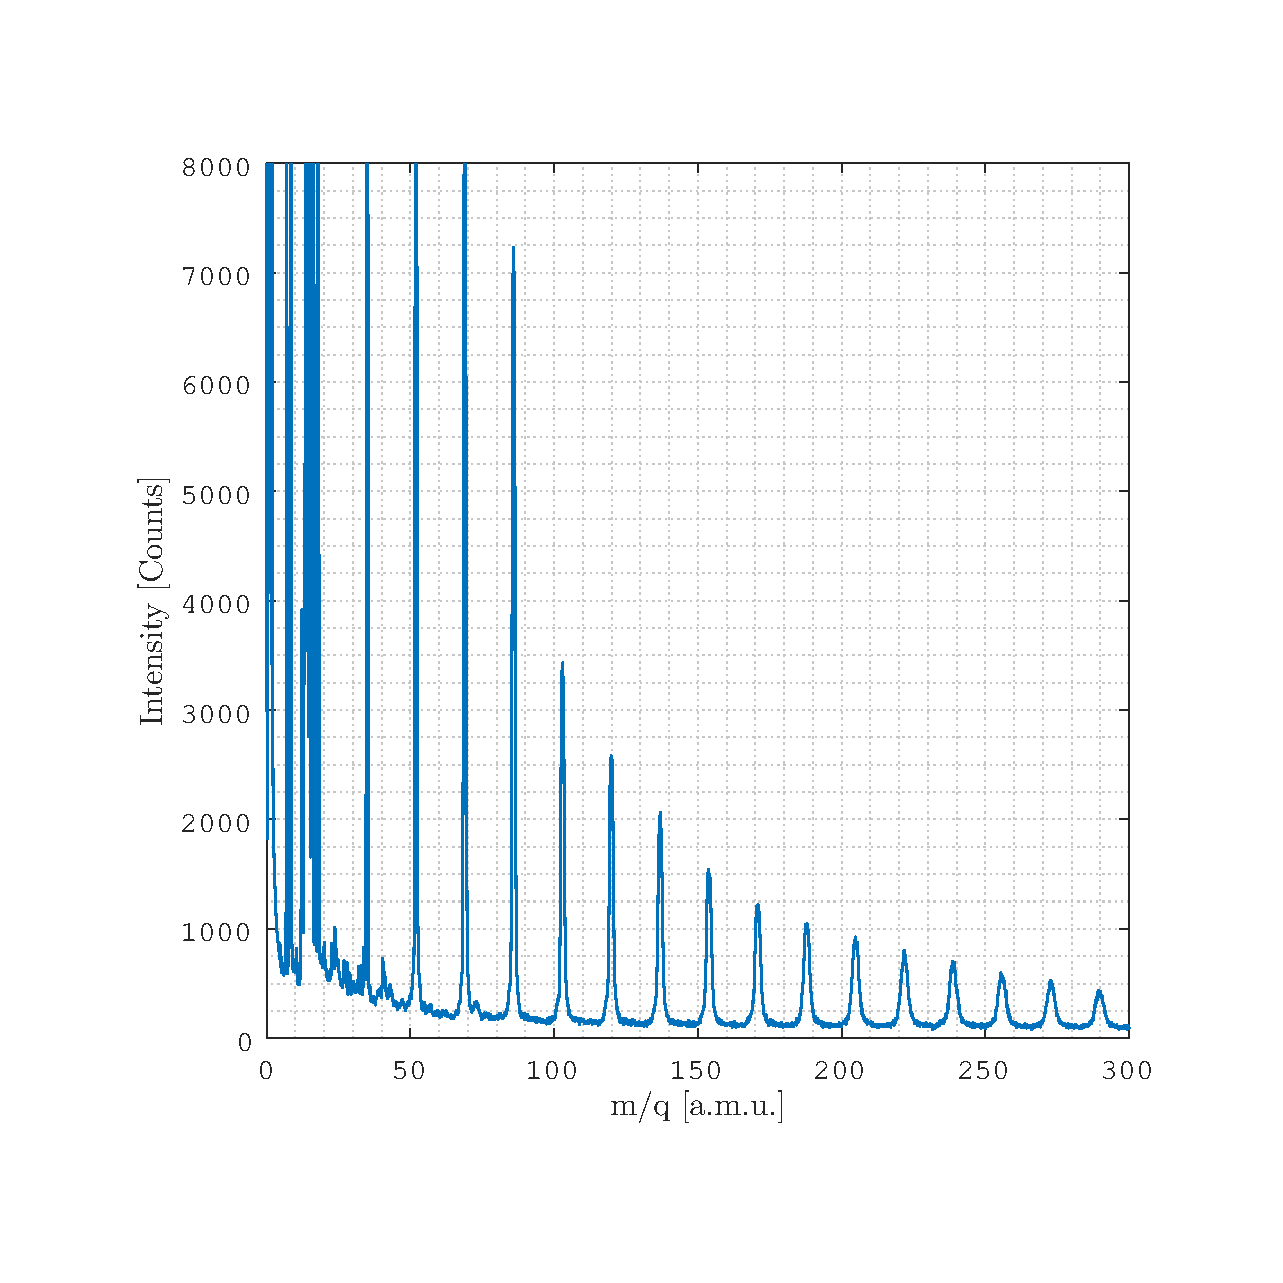
\includegraphics[width=0.9\textwidth]{Graphics/m2q_hist_example.eps}}
\caption{Example of a mass-to-charge histogram of pure NH$_3$-clusters from a molecular beam.}
\end{figure}

\subsubsection{momentum}

\newpage
\subsection{calibrate}
The calibrate functions go through a procedure that return correct correction and conversion factors. These should afterwards be stored in the metadata, category `conversion factors'. 

\paragraph{TOF $\rightarrow m/q$ factor}

\paragraph{detection center position}

\paragraph{detector rotation}

\paragraph{residual momentum minimualization}
The residual momentum of a two-body process, resulting in two cations, can be used to calibrate the spectrometer. This module minimizes the relative norm of the residual momentum:

\begin{align}
f_{min} = \frac{norm(\vec{p}_{res})}{norm(\vec{p}_{1} - \vec{p}_{2})} = \frac{norm(\vec{p}_{1} + \vec{p}_{2})}{norm(\vec{p}_{1} - \vec{p}_{2})}
\end{align}

The variables that are tweaked during this optimization:

\begin{itemize}
\item corr.det1.dX	(X-shift of the raw image)
\item corr.det1.dY (Y-shift of the raw image)
\item spec.volt.Ve2s (voltage of grid between electron MCP and source ('pusher'))
\item conv.det1.TOF\_2\_M2Q.factor (Conversion factor from mass 2 charge to TOF) 
\item conv.det1.TOF\_2\_M2Q.t0 (time correction)
\end{itemize}

This function requires the input values to be roughly calibrated, so should be used as a final calibration: the solver only searches in a small solution domain and only a local minimum is found. 

\begin{figure}[H]
   \centering
    \centerline{\includegraphics[width=0.9\textwidth]{Graphics/MB_calib.png}}
\caption{Example of a molecular beam calibration}
\label{MB_calib}
\end{figure}

\newpage
\subsection{general}
Functions of general use are stored in this category, that are outside of the standard package of MATLAB. These can be written for the package, and of use for all package categories. They can also originate from MATLAB File Exchange (\url{http://nl.mathworks.com/matlabcentral/fileexchange/}) 
The package has no parameters or constants stored, they are in general all provided by the metadata (see section 'metadata structure'). An exception is the general constants of nature, that are more or less written in stone. For example the unit conversion factors (converting eV to Joule). These constants are also stored in this category.



\lstset{language=MATLAB}
\begin{lstlisting}
% Example of MATLAB codes/functions
[input1, input2] = function test(input1, input2)
\end{lstlisting}

\if
% Remarks from meeting Shabnam and Noelle 17th of september:
-make TOF to m2q not only by clicking, also by typing numbers.
Make it possible to look at the corresponding NEXAFS/total ion yield spectra also
think about the best way of determining the center of detection, which is now done by eye.
make it possible to subtract background for the converted energies from an off-resonance measurement
make it possible to calculate the beta-parameter of only a certain range of kinetic energy releases.
store all the converted values so that it can be used later.
PEPIPICO plots in m/q units instead of TOF.
don't do the m/q labeling automatically; it is best to do this manually.
combining events from different measurements is very useful. maybe also selecting a certain KE from a measurement and saving that as a separate measurement?
maybe make it possible to look at branching ratio's of different measurements?
Could the beta-parameter be determined when only part of the detector region is used?
make binsize user-adjustable
make it possible to histogram any variable against another. Maybe; define binsize for every signal.
look up how to print horizontal lines in text.
\fi

%\newpage
\section{Diagnostics}

\subsection{Theory}

For electrostatic spectrometers, 'dummy data' can be created. The Time Of Flight of one section is calculated by solving the following polynomial equation:


\begin{equation}
\tfrac{1}{2} \cdot q \cdot E \cdot TOF^2 + p_{ini} \cdot TOF
\end{equation}


\subsection{SIMION}



\section{Installation}
\input{../../README.md}

\end{document}
